%!TEX root = ../thesis.tex
% ******************************* Thesis Appendix A2 ********************************

\ifpdf
\graphicspath{{chapter-background/Figs/Raster/}{chapter-background/Figs/PDF/}{chapter-background/Figs/}}
\else
\graphicspath{{chapter-background/Figs/Vector/}{chapter-background/Figs/}}
\fi

\section{Background estimation}\label{app:background_estimation}
\begin{figure}[H]
	\centering
	\begin{subfigure}[b]{0.5\linewidth}
		\centering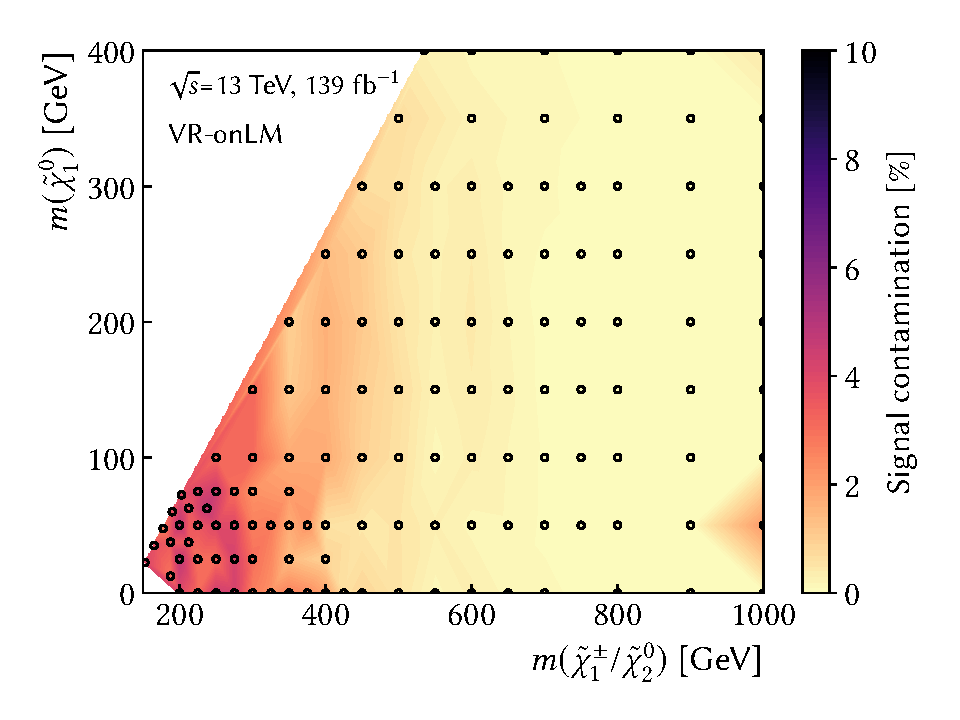
\includegraphics[width=1.0\textwidth]{signal_contamination/plot_VR_onLM}
		\caption{VR-onLM\label{fig:signal_contamination_VRon1}}
	\end{subfigure}\hfill
	\begin{subfigure}[b]{0.5\linewidth}
		\centering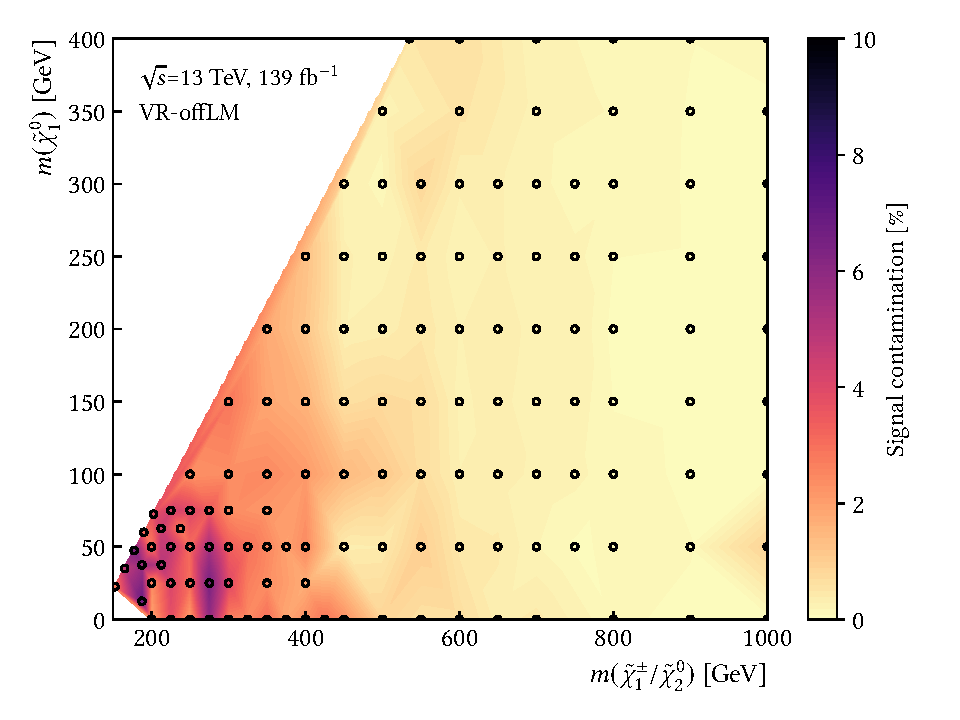
\includegraphics[width=1.0\textwidth]{signal_contamination/plot_VR_offLM}
		\caption{VR-offLM\label{fig:signal_contamination_VRoff1}}
	\end{subfigure}\hfill
	\par\medskip
	\begin{subfigure}[b]{0.5\linewidth}
		\centering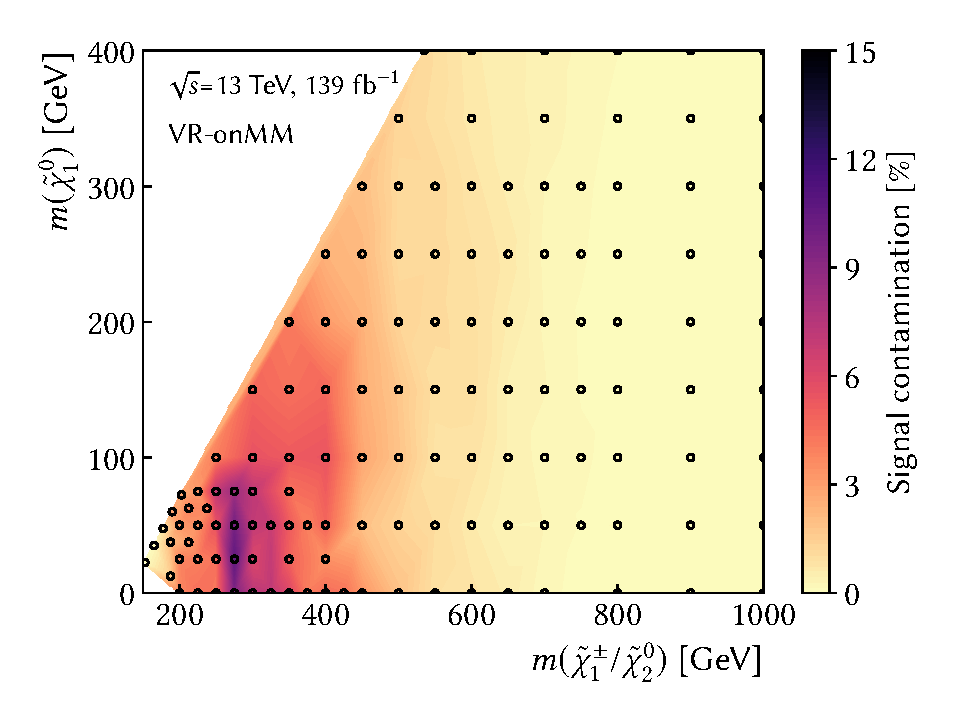
\includegraphics[width=1.0\textwidth]{signal_contamination/plot_VR_onMM}
		\caption{VR-onMM\label{fig:signal_contamination_VRon2}}
	\end{subfigure}\hfill
	\begin{subfigure}[b]{0.5\linewidth}
		\centering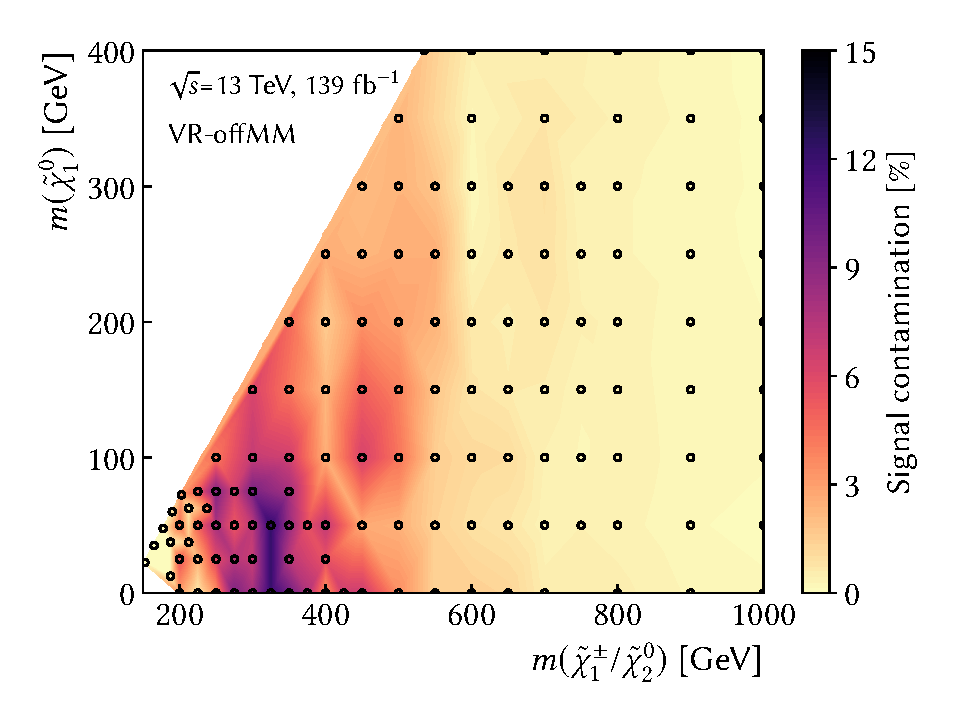
\includegraphics[width=1.0\textwidth]{signal_contamination/plot_VR_offMM}
		\caption{VR-offMM\label{fig:signal_contamination_VRoff2}}
	\end{subfigure}\hfill
	\begin{subfigure}[b]{0.5\linewidth}
		\centering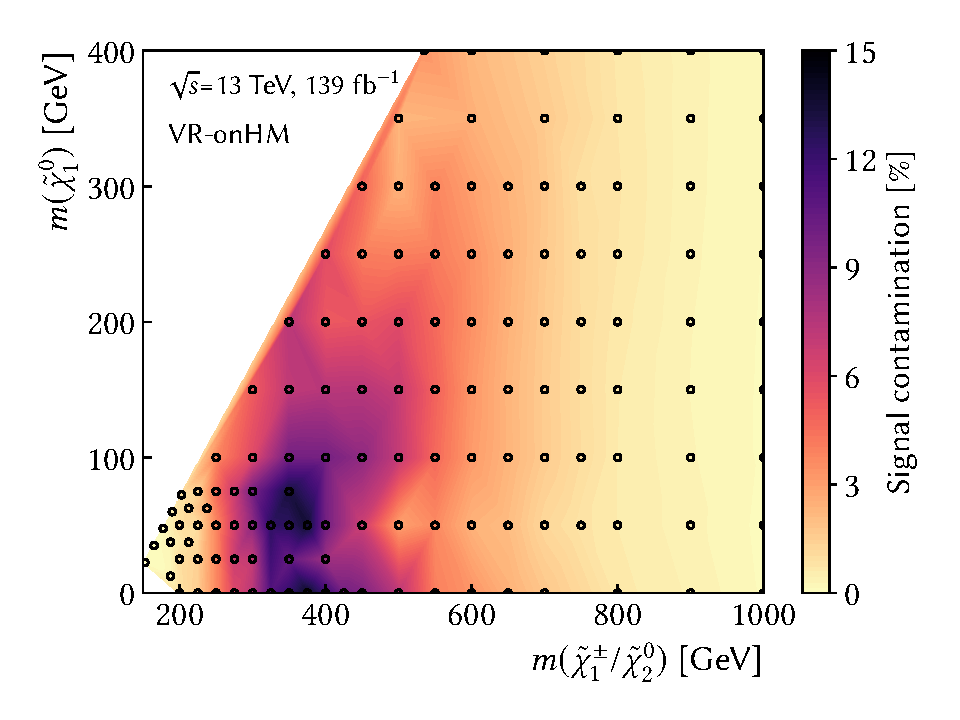
\includegraphics[width=1.0\textwidth]{signal_contamination/plot_VR_onHM}
		\caption{VR-onHM\label{fig:signal_contaminations_VRon3}}
	\end{subfigure}\hfill
	\begin{subfigure}[b]{0.5\linewidth}
		\centering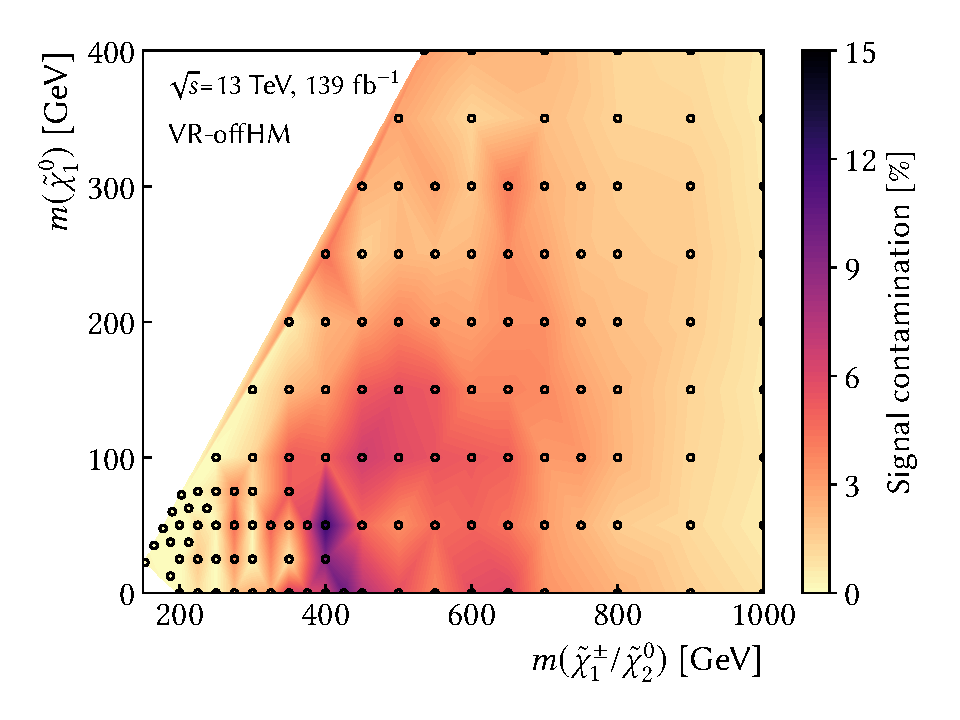
\includegraphics[width=1.0\textwidth]{signal_contamination/plot_VR_offHM}
		\caption{VR-offHM\label{fig:signal_contaminations_VRoff3}}
	\end{subfigure}\hfill

	\caption{Signal contamination (shown on the \textit{z-axis}) for all \glspl{vr} throughout the signal grid. The space between the signal points (indicated by the black circles) is interpolated using Delaunay triangles.}
	\label{fig:signal_contaminations_VRs}
\end{figure}



\ifpdf
\graphicspath{{chapter-results/Figs/Raster/}{chapter-results/Figs/PDF/}{chapter-results/Figs/}}
\else
\graphicspath{{chapter-results/Figs/Vector/}{chapter-results/Figs/}}
\fi


\begin{sidewaysfigure}[ht]
	\centering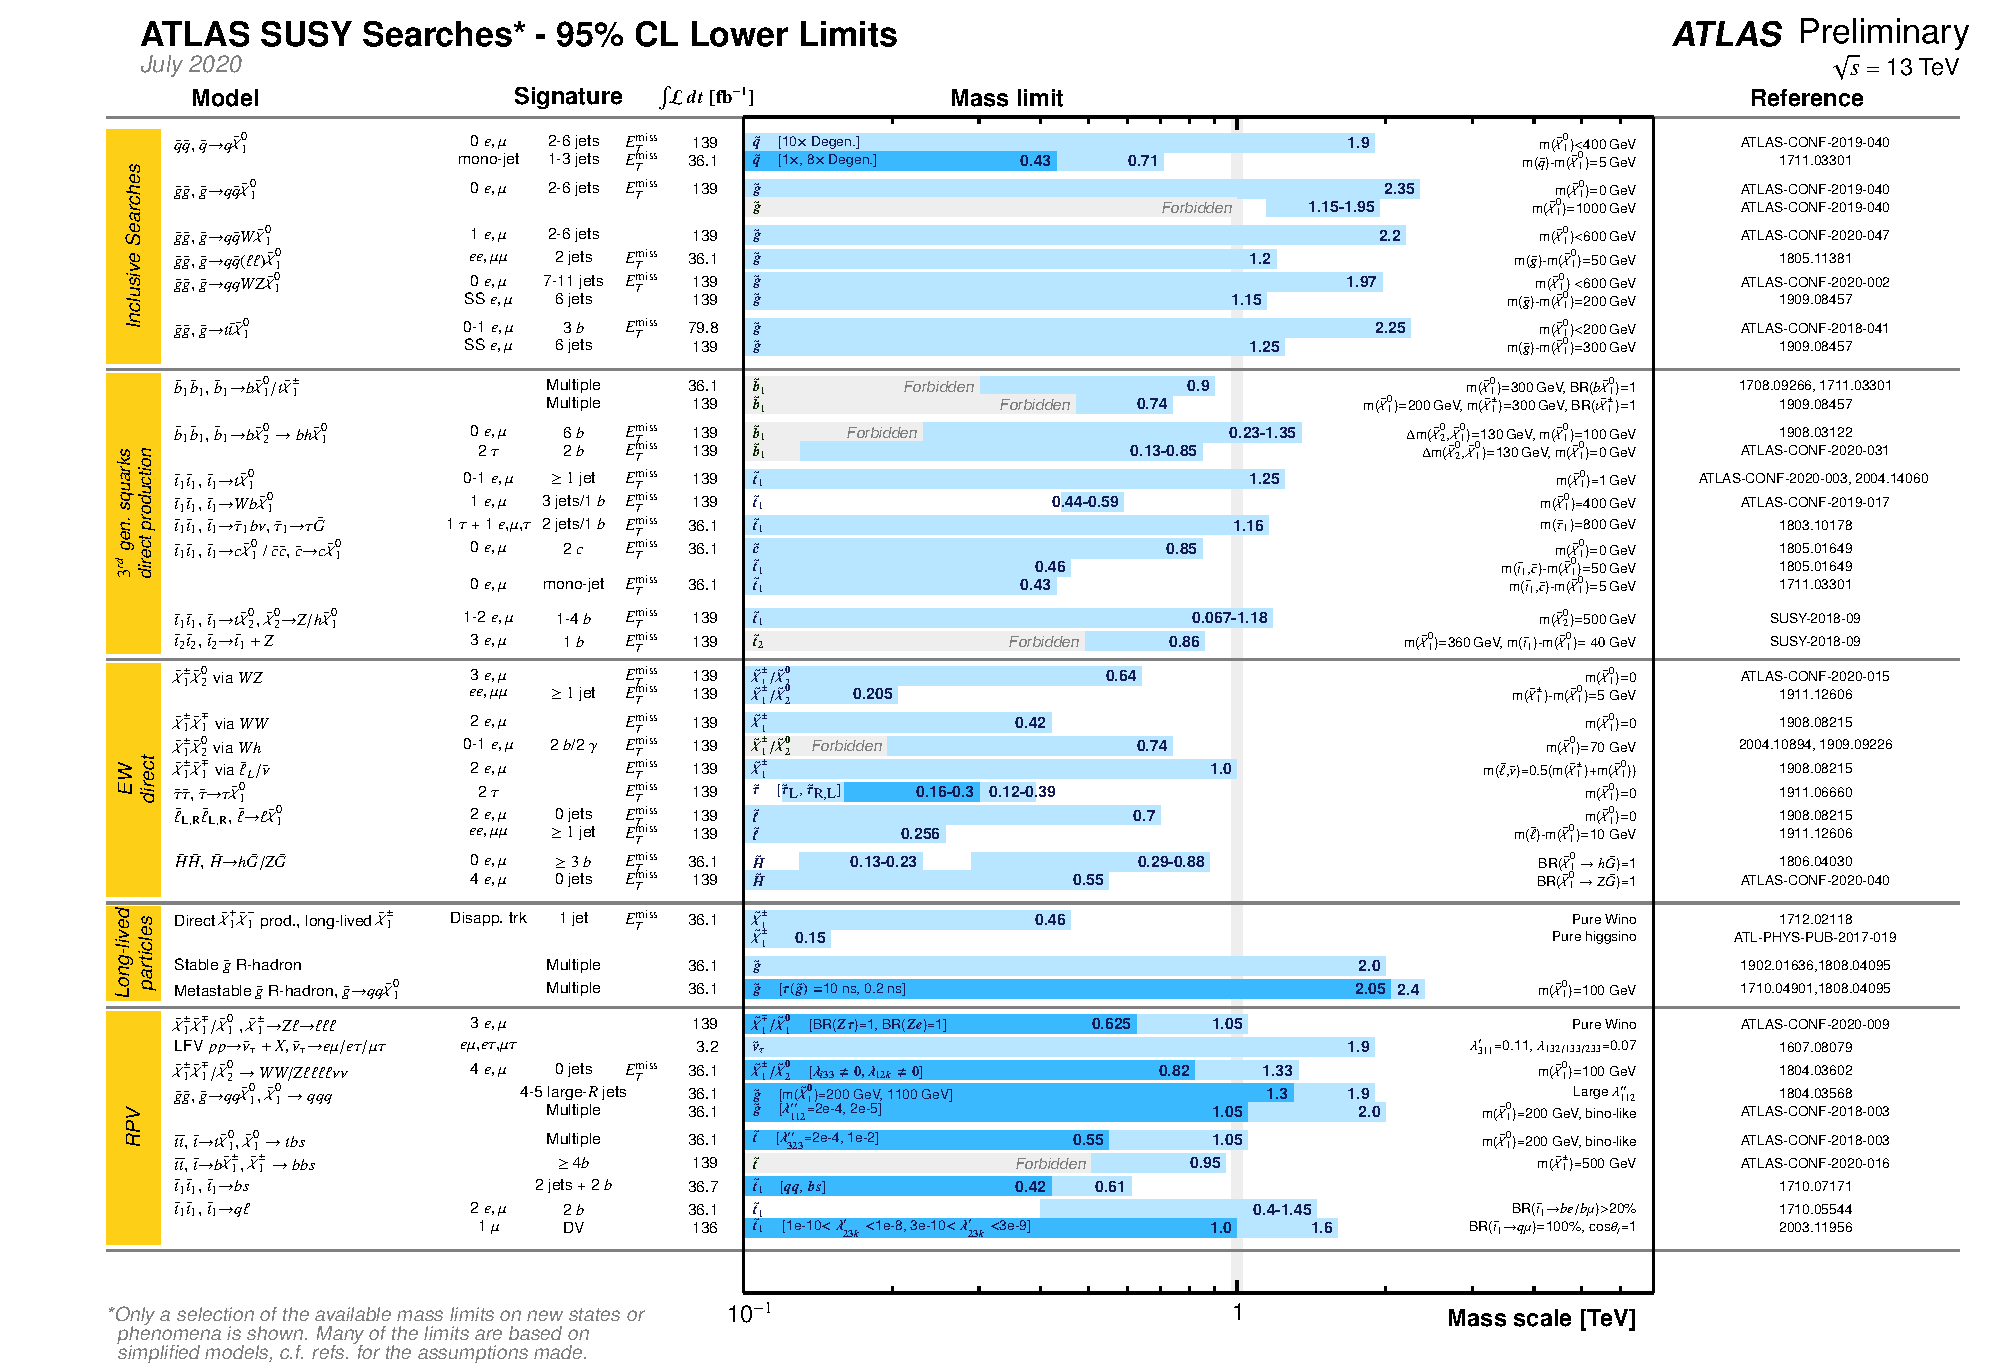
\includegraphics[width=0.9\textwidth]{susy_summary}
	\caption{Summary of the ATLAS searches for \gls{susy}. A representative selection of the available search results is shown. Results are given with respect to the nominal cross section. In some cases these additional dependencies are indicated by darker bands showing different model parameters. Figure adapted from \reference\cite{ATL-PHYS-PUB-2020-020}.}
	\label{fig:susy_summary_plot}
\end{sidewaysfigure}
